\subsection{Outdoor sound field model}
Outdoor sound has been a subject of investigation for a long time. Initial investigations were concerned with ascertaining the speed of sound. We have come a long way since then, whereupon it is of interest to predict the complex sound field behaviour outdoors. This is to solve the two-part problem of first, measuring urban noise levels, and second, finding their major contributors. The second part of the problem is solved using source localization algorithms discussed in later sections, which can be used to 'localize' the sound received at a microphone array to its actual source. However, before tackling the problem of outdoor sound localization, the sound field behaviour outdoors needs to be understood. A variety of factors affect outdoor sound propagation like the ground (earth), atmospheric absorption, barriers between line-of-sight to the sound source, wind, temperature, turbulence etc.

Various different models have been designed for outdoor sound field received at a receiver. The ISO 9613-2 \cite{ISO9613} is an international standard model for attenuation of sound when propagating outdoors. The standard uses an empirical method to quantify attenuation in different circumstances. This is a disadvantage as the model might not fit particular real world scenarios and user discretion is needed when using the model. NMPB-2008 \cite{dutilleux2010nmpb} is a French standard model which uses simple engineering methods to model road traffic noise. Over time it has been extended to include other sound sources. Nord2000 \cite{plovsing2000nord2000} and Harmonoise \cite{defrance2007outdoor} are more advanced engineering models for outdoor sound propagation. Nord2000 was developed in the period 1996-2001 by DELTA (Denmark, project manager, SINTEF (Norway), and SP (Sweden). Harmonoise is a more recent method and is made with a collaboration of various European countries. Nord2000 and Harmonoise are based on a similar approach and often produce quite similar models. Various inconclusive studies have been conducted comparing the two \cite{garg2014critical},\cite{jonsson2008comparison}. Eventually, to have a harmonized and coherent approach, a common framework for noise assessment (CNOSSOS-EU) was developed by the European Commission \cite{kephalopoulos2012common} in co-operation with the EU Member States to be applied for strategic noise mapping as required by the Environment Noise Directive (2002/49/EC). CNOSSUS-EU investigates the various existing methods and their advantages and disadvantages. It takes into consideration the accuracy as well as the computational complexities of the various methods. 
In general, the factors affecting outdoor sound propagation are described below.

\subsubsection{Spreading loss} 
The sound intensity from an omni-directional sound source drops as a function of distance due to wavefront spreading. The intensity I at distance r of a source with power P, is given by
\begin{equation}
    I = \frac{P}{4\pi r^2}.
\end{equation}
This is due to spherical propagation, where the surface of the sphere has area $4\pi r^2$. In logarithm form this becomes
\begin{equation}
\begin{split}
    10log(I) &= 10log(\frac{P}{4\pi r^2}) \\
    L_p &= L_w - 20 log(r) - 11,
\end{split}
\end{equation}
which means a reduction of $20log2 = 6 dB$, every doubling of r. This equation assumes uniform omni-directional directivity. For directional sources a Directivity Index DI can be added giving
\begin{equation}
    L_p = L_w + DI - 20 log(r) - 11.
\end{equation}
It is important to remember that such a directivity can be inherent to the source or might be induced due to the location of the source. An omni-directional source placed on a perfectly reflecting plane can only propagate sound into a hemisphere, in which case the DI is 3 dB.  
An infinite line source can be viewed as an linear array of omni-directional point sources. The wavefront spread is cylindrical (surface area $= 2\pi r$),  which gives 
\begin{equation}
\begin{split}
    10log(I) &= 10log(\frac{P}{2\pi r}) \\
    L_p &= L_w - 10 log(r) - 8,
\end{split}
\end{equation}
and the reduction is $10log2 = 3$ dB, every doubling of r. Highway traffic is modelled in a similar manner, assuming 3 dB drop every doubling of distance.

\subsubsection{Atmospheric absorption}
Sound energy converts to heat as it travels through the air. The portion of sound absorbed by air becomes increasingly important as distance of propagation increases. For a plane wave, the loudness L at a distance x from a position of known loudness $L_0$ is given by
\begin{equation}
    L= L_0 - k.x,
\end{equation}
where k depends on the humidity, temperature, pressure as well as the molecular composition of atmosphere and is a function of frequency. k is given by
\begin{equation}

\end{equation}


k is a quadratic function of frequency, so higher frequencies are absorbed more. This causes air to act as a low-pass filter over large distances. 
The conversion of sound to heat can happen due to conduction, shear viscosity or by molecular relaxation. Molecular relaxation \cite{bass1990atmospheric}, \cite{evans1972atmospheric} is an important factor with losses due to oxygen-water vapour molecular relaxation being predominant above 500Hz, being atleast 2 dB/kilometer and increasing rapidly with frequency. The total absorption below 200 Hz is less than 1 dB/kilometer and decreases with frequency. If the air is extremely dry ($< 10\%$ relative humidity), the oxygen-carbon dioxide relaxation becomes significant and causes an almost constant absorption down from 500Hz to 80Hz of around 2dB/kilometer. The total air absorption as a function of frequency can be seen in Fig. \ref{Fig:airAbsorption}.

\begin{figure}
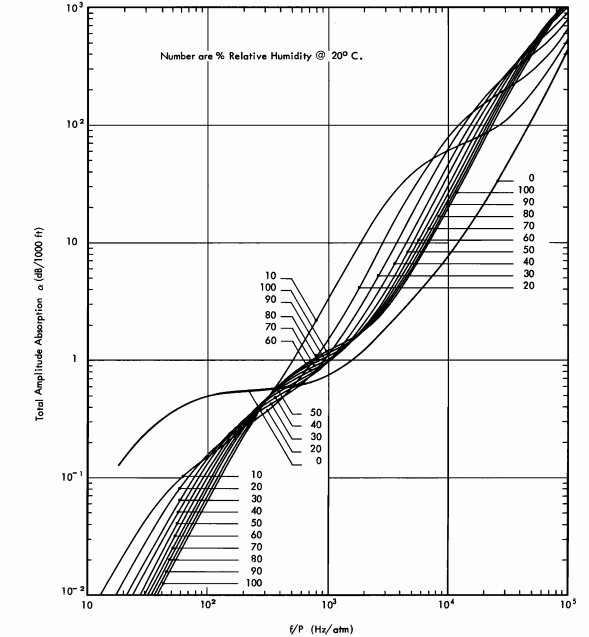
\includegraphics[width=0.8\textwidth]{Figures/airAbsorption.png}
\caption{Total absorption of sound in air as a function of frequency. The curves range from 0 to 100\% relative humidity and are for 20\degree C \cite{evans1972atmospheric} (Notice that the y-axis units are per 1000ft).}
\label{Fig:airAbsorption}
\end{figure}

\subsubsection{Diffraction and barriers}
Barriers are sometimes purposefully built to block the direct path from the sound source to the receiver. Sound then reaches the receiver either going through the barrier or by diffracting around the top of the barrier. Of course this only works as long as the receiver is actually below the barrier height. Ground reflections and multi-path-propagation may lead to multiple diffracted wave paths. For a barrier, the ISO 9613-2 \cite{ISO9613} provides the following equation for loss due to barrier insertion
\begin{equation}
    IL = 10log\bigg[3+\bigg(C_2\frac{\delta_1}{\lambda}\bigg)C_3K_{met}\bigg],
\end{equation}
where the value of $C_2$ determines if ground reflections are taken care of($C_2 = 20$) or not($C_2 = 40$), $C_3$ is a factor to take care of double diffraction due to a barrier of finite thickness (or two thin barriers placed some distance apart), $\delta_1$ is the difference in distance between the direct source-to-receiver path and the wave propagation path due to the barrier, and $K_{met}$ is a correction factor for average downwind meteorological effects. The equation simplifies to 
\begin{equation}
    IL = 10log(3+40\frac{\delta_1}{\lambda}), 
\end{equation}
for thin barriers.